\documentclass[11pt]{article}

% ---- Packages (all standard; MiKTeX will auto-install if missing) ----
\usepackage[utf8]{inputenc}
\usepackage[T1]{fontenc}
\usepackage{lmodern}        % scalable Type1 fonts (required for microtype expansion)
\usepackage[margin=1in]{geometry}
\usepackage{amsmath,amssymb}
\usepackage{booktabs}
\usepackage{graphicx}
\usepackage{xcolor}
\usepackage{microtype}
\usepackage{enumitem}
\usepackage{caption}
\usepackage[numbers,sort&compress]{natbib}
\usepackage[hidelinks]{hyperref}

\graphicspath{{figures/}}
\newcommand{\guidance}{\textsc{guidance}}
\newcommand{\context}{\textsc{context}}
\newcommand{\cmark}{\textcolor{green!55!black}{$\checkmark$}}
\newcommand{\xmark}{\textcolor{red!70!black}{$\times$}}

\title{\textbf{Policy-Guided RAG: Asymmetric Visibility\\ for Controllable Retrieval}}
\author{Jainil Gosalia\\\small Independent Researcher}
\date{June 2026}

\begin{document}
\maketitle

\begin{abstract}
Retrieval-Augmented Generation (RAG) systems cannot currently enforce hidden business rules
or safety constraints during retrieval without exposing those rules to the LLM. We introduce
\textbf{Policy-Guided RAG}, a retrieval architecture built on an \emph{asymmetric visibility}
pattern: hidden \guidance{} chunks influence ranking, but are physically filtered before LLM
generation, so they are \emph{structurally absent} from the model's context rather than merely
hidden. We study two mechanisms for letting guidance steer ranking. The intuitive
\emph{query-augmentation} mechanism --- appending guidance text to the query before
cross-encoder reranking --- \emph{does not work}: on a benchmark whose relevance labels are
constructed independently of the guidance, it yields no steering, and on a hand-verified set
it significantly \emph{degrades} ranking ($p{=}0.039$). A topical cross-encoder cannot
interpret ``avoid card $X$'' as a down-weight, so negative guidance is inexpressible this way.
We then introduce an explicit \emph{policy operator} that applies structured
\textsc{boost}/\textsc{demote}/\textsc{exclude} actions to the reranked scores. The operator
delivers large, statistically significant control --- a \textsc{boost} steering lift of
$+27.6$ ranks (95\% CI $[+21.2,+34.1]$) and a reduction in excluded-card appearance from
$51.7\%$ to $6.9\%$ ($\to 0\%$ with fuller guidance retrieval) --- at no measurable relevance
cost at the default operating point, and a tunable control--relevance trade-off beyond it.
Across both mechanisms a $185$-query audit (manual, synthetic, and adversarial) repeated over
all mechanisms ($555$ runs) finds \textbf{zero} guidance leakage. Our contributions are the
asymmetric-visibility guarantee, the policy operator, a non-circular evaluation protocol, and
the negative result on query augmentation.

\vspace{4pt}
\noindent\textbf{Keywords:} Retrieval-Augmented Generation, Information Retrieval, Policy
Enforcement, Cross-Encoder Reranking, Hidden Constraints.
\end{abstract}

\section{Introduction}
Retrieval-Augmented Generation (RAG) systems enhance Large Language Model (LLM) responses by
retrieving relevant context from external knowledge bases \citep{lewis2020rag,guu2020realm}.
While RAG has proven effective for factual grounding and knowledge-intensive tasks, current
systems cannot enforce hidden business rules or safety constraints during retrieval.

\subsection{Problem Statement}
Consider a credit card recommendation chatbot that must: (1)~prioritize specific cards for
business queries (hidden strategy), (2)~avoid recommending high-fee cards to fee-sensitive
users (hidden policy), and (3)~comply with regulatory requirements invisibly (hidden
compliance). Current RAG systems have no mechanism to apply such rules without either
exposing them to the LLM (jailbreakable, visible in logs), filtering content entirely (too
rigid, binary yes/no), or making multiple LLM calls (expensive, slow). The fundamental
limitation is that standard RAG treats all retrieved content equally --- there is no way to
use hidden policy information to influence what gets ranked highly without exposing that
policy to the LLM or end user.

\subsection{Our Approach}
We introduce Policy-Guided RAG, a retrieval architecture that lets hidden business rules and
safety constraints influence ranking without ever exposing them to the LLM. The core is an
\emph{asymmetric visibility} pattern: guidance influences the ranking process but is physically
removed before generation. We compare two mechanisms for applying guidance --- query
augmentation and an explicit policy operator --- and find that only the operator achieves
controllable ranking. The system operates in stages: (1)~\emph{dual retrieval} of content and
guidance chunks; (2)~a guidance mechanism (augment the query, \emph{or} apply the operator);
(3)~\emph{cross-encoder reranking}; (3.5)~the \emph{policy operator} when enabled; and
(4)~\emph{post-rerank filtering} that removes guidance before LLM generation.
Figure~\ref{fig:arch} illustrates the architecture.

\begin{figure}[t]
\centering
\noindent\rule{\linewidth}{0.4pt}
{\footnotesize
\begin{verbatim}
User query q
   |-- vector search WHERE chunk_type = "context"  -> k_c candidate context chunks
   |-- vector search WHERE chunk_type = "guidance"  -> k_g guidance chunks (HIDDEN)
            |
            v   cross-encoder re-rank:  score(q, c_i)  for each candidate c_i
            v   policy operator:  +w BOOST / -w DEMOTE / drop EXCLUDE targets
            |   (alt. mechanism: augment q with guidance text before reranking)
            v   sort by score  ->  keep only chunk_type == "context"  ->  top-n
   final context  -- guidance physically removed -->  LLM generation
\end{verbatim}
}
\noindent\rule{\linewidth}{0.4pt}
\caption{Policy-Guided RAG architecture. Guidance influences reranking but is physically
removed before LLM generation, guaranteeing zero information leakage.}
\label{fig:arch}
\end{figure}

\subsection{Contributions}
\begin{itemize}[leftmargin=1.4em,itemsep=2pt]
  \item \textbf{Asymmetric visibility guarantee:} guidance affects the \emph{process}
  (reranking) but is structurally absent from the \emph{product} (LLM context); verified
  leak-free across 185 queries $\times$ 3 mechanisms (555 runs).
  \item \textbf{Policy operator:} an explicit \textsc{boost}/\textsc{demote}/\textsc{exclude}
  mechanism that yields large, significant, and exact ranking control
  (\textsc{boost} steering lift $+27.6$; \textsc{exclude} enforcement to $0\%$) with no
  off-the-shelf training, at a tunable relevance cost.
  \item \textbf{Negative result:} the intuitive query-augmentation mechanism does not steer
  retrieval and can significantly degrade it, with a mechanistic explanation.
  \item \textbf{Non-circular evaluation protocol:} relevance labels derived independently of
  guidance, with separate controllability/enforcement metrics and paired significance tests.
  \item \textbf{Generality via attribute predicates:} the same operator governs a document
  corpus under a hidden records schedule using attribute predicates (not item IDs), so policies
  need no per-item coding and survive corpus drift.
  \item \textbf{Open source:} complete implementation and datasets for reproducibility.
\end{itemize}

\subsection{Motivation and Applications}
Policy-Guided RAG enables two broad categories of applications. \textbf{Business logic \&
recommendations:} e-commerce (promote profitable products invisibly), content platforms
(apply regional compliance rules), financial services (enforce GDPR/SOC2), healthcare
(HIPAA-compliant filtering). \textbf{Safety \& guardrails:} jailbreak-resistant filtering
(the LLM never sees the rules), proactive content safety, and addressing the ``RAG makes
guardrails unsafe'' vulnerability \citep{robey2024rag}.

\section{Related Work}

\subsection{Retrieval-Augmented Generation}
RAG was introduced to address LLMs' limitations in knowledge grounding and factual accuracy
\citep{lewis2020rag}. Since then, dense retrieval \citep{karpukhin2020dpr}, bi-encoders
\citep{reimers2019sbert}, hybrid BM25$+$neural approaches \citep{robertson2009bm25}, and
advanced strategies such as Self-RAG \citep{asai2023selfrag} and query rewriting
\citep{ma2023query} have become standard. However, all of these approaches treat retrieved
content equally --- there is no mechanism for hidden policy enforcement.

\subsection{Cross-Encoder Reranking}
Cross-encoders have become essential for improving retrieval quality beyond bi-encoder
similarity \citep{nogueira2019passage}. The MS~MARCO dataset \citep{nguyen2016msmarco}
enabled training effective cross-encoders; BGE-reranker \citep{xiao2023cpack} achieves SOTA
on BEIR \citep{thakur2021beir}. Our work applies cross-encoders in a novel way: not just for
relevance scoring, but for policy-enforced ranking through query augmentation.

\subsection{Controllable Generation and Safety}
System prompts, guided generation, and RLHF/DPO \citep{ouyang2022instruct,rafailov2024dpo}
all control LLM outputs at generation time. Our approach is orthogonal: we control retrieval
rather than generation. Recent work has identified vulnerabilities in RAG-based systems ---
``RAG makes guardrails unsafe'' \citep{robey2024rag} demonstrates that standard RAG can
bypass safety mechanisms. Our approach addresses these concerns by keeping policy rules
entirely invisible to the LLM.

\subsection{Comparison with Alternative Approaches}
Table~\ref{tab:compare} compares Policy-Guided RAG with alternatives on four key desiderata.
Our approach is the only one satisfying all four simultaneously.

\begin{table}[h]
\centering
\begin{tabular}{lcccc}
\toprule
Approach & Hidden & Flexible & Single Call & Jailbreak-Resistant \\
\midrule
System prompt            & \xmark & \cmark & \cmark & \xmark \\
Post-filtering           & \cmark & \xmark & \cmark & \cmark \\
Multi-stage LLM          & \cmark & \cmark & \xmark & \xmark \\
\textbf{Policy-Guided RAG (ours)} & \cmark & \cmark & \cmark & \cmark \\
\bottomrule
\end{tabular}
\caption{Comparison with alternative approaches. Policy-Guided RAG is the only method
satisfying all four desiderata.}
\label{tab:compare}
\end{table}

\section{Method}

\subsection{Problem Formulation}
Let the vector database contain context chunks $C=\{c_1,\dots,c_n\}$ (visible to the LLM) and
guidance chunks $G=\{g_1,\dots,g_m\}$ (hidden from the LLM). Given a user query $q$, the goal
is to retrieve the top-$k$ context chunks that respect the constraints in $G$. Traditional
RAG ignores $G$ entirely. Our approach augments $q$ with retrieved $G$, reranks using a
cross-encoder, then filters $G$ before LLM generation --- creating an asymmetric visibility
pattern.

\subsection{Stage 1: Dual Retrieval}
Context retrieval fetches the top-$k_1{=}10$ most semantically similar content chunks.
Guidance retrieval fetches the top-$k_2{=}3$ most relevant policy rules. Separate retrieval
via metadata filtering prevents guidance from polluting content ranking and allows each type
to be optimized independently.

\subsection{Stage 2: Two Guidance Mechanisms}
We study two ways for retrieved guidance to influence ranking.

\textbf{(a) Query augmentation.} The augmented query is constructed as
$q' = q \,\Vert\, \texttt{[GUIDANCE]} \,\Vert\, g_1 \,\Vert\, g_2 \,\Vert\, \cdots$ and scored
by the cross-encoder. This is the intuitive mechanism, but it can only \emph{add} topical
signal: a cross-encoder estimates relevance between $q'$ and a document, so appending ``avoid
card $X$'' tends to \emph{raise} card $X$'s score (it mentions $X$), not lower it. Negative
guidance is therefore inexpressible, and \S\ref{sec:results} shows even positive guidance does
not reliably steer ranking this way.

\textbf{(b) Policy operator.} Each guidance rule carries a structured action
$a \in \{\textsc{boost},\textsc{demote},\textsc{exclude}\}$ and a set of target cards $T$.
After the cross-encoder scores candidates against the \emph{raw} query, the operator adjusts
scores directly: $s(c) \mathrel{+}= w$ for $c \in T$ under \textsc{boost}, $s(c) \mathrel{-}= w$
under \textsc{demote}, and $c$ is removed entirely under \textsc{exclude}. \textsc{boost}
targets absent from the candidate pool are injected (fetched by id and scored) so policy can
surface a card embedding similarity missed. \textsc{exclude} is a structural removal, hence
exact for any retrieved rule.

\subsection{Stage 3: Cross-Encoder Reranking}
Cross-encoders process query and document jointly:
$\operatorname{score}(q, c_i) = \operatorname{model}([q, c_i])$, giving full cross-attention
between them. Under mechanism (a) the augmented query $q'$ is used; under mechanism (b) the raw
query $q$ is used and policy is applied in Stage 3.5. We use
\texttt{cross-encoder/ms-marco-MiniLM-L-6-v2} (22M parameters, MS~MARCO passage ranking) as
the default reranker.

\subsection{Stage 3.5: Policy Operator (mechanism b)}
When the operator is enabled, it is applied to the reranked candidate list as described above,
before filtering. Because it manipulates only \context{} scores and removals (never injecting
\guidance{} into the candidate set), it leaves the zero-leakage guarantee intact.

\subsection{Stage 4: Post-Rerank Filtering}
Guidance chunks are physically removed before LLM generation by retaining only chunks where
\texttt{metadata['chunk\_type'] == 'context'}. This guarantees zero leakage even under
adversarial jailbreak attempts or context-injection attacks --- the guidance is
\emph{structurally absent}, not merely hidden.

\subsection{Why the Operator, Not Augmentation}
A cross-encoder scores topical relevance, so the augmented-query mechanism can only push
\emph{toward} terms present in the query; it has no way to enforce a preference ordering or a
prohibition. The explicit operator instead treats guidance as what it is --- a ranking
constraint --- and applies it to the scores. This makes positive, negative, and hard-exclusion
policies all expressible and exact (for \textsc{exclude}), at the cost of an explicit
strength parameter $w$ that trades policy compliance against relevance (\S\ref{sec:results}).

\section{Experiments}

\subsection{Research Questions}
\begin{itemize}[leftmargin=1.4em,itemsep=1pt]
  \item \textbf{RQ1:} Does the query-augmentation mechanism let guidance steer retrieval?
  \item \textbf{RQ2:} Does the explicit policy operator achieve controllable ranking
        (\textsc{boost}/\textsc{demote}/\textsc{exclude}) without harming relevance?
  \item \textbf{RQ3:} What is the trade-off between policy enforcement and relevance?
  \item \textbf{RQ4:} Does guidance information leak into LLM-visible outputs?
  \item \textbf{RQ5:} Does the approach generalize beyond cards to document governance with
        attribute-predicate policies?
\end{itemize}

\subsection{Datasets}
\textbf{Manual test set (high quality):} 15 hand-verified queries, 15 credit cards, 7 free-text
guidance rules. Queries cover lounge access, student cards, business cards, fee sensitivity,
and credit-score requirements. Because the guidance is free text (no structured action), only
the augmentation mechanism applies here.
\textbf{Synthetic test set (large scale):} 150 template-generated queries, 50 credit cards, 27
structured guidance rules (19 \textsc{boost}, 6 \textsc{demote}, 2 \textsc{exclude}). Difficulty
distribution: 30/35/25/10\% easy/medium/hard/expert. Generated and validated deterministically
(seed 42) by \texttt{src/data\_generation}.

\paragraph{Non-circular labels.} Relevance gold (\texttt{expected\_top\_cards}) is derived
\emph{only} from card attributes matched to the query category, independently of the guidance
rules; ambiguous/adversarial queries carry empty gold and are excluded from accuracy. Guidance
influence is measured by separate fields --- \texttt{policy\_preferred\_cards} (\textsc{boost}
targets) and \texttt{policy\_excluded\_cards} (\textsc{exclude} targets) --- never used as
relevance gold. This avoids the circularity of letting the guidance define the very labels the
method is scored against.

\subsection{Evaluation Metrics}
\emph{Accuracy:} Top-1/Top-5 and mean position on the relevance-labelled subset.
\emph{Controllability (\textsc{boost}):} mean rank and top-$n$ hit-rate of
\texttt{policy\_preferred\_cards}, and a \emph{steering lift} (rerank-only rank minus condition
rank) with a bootstrap 95\% CI. \emph{Enforcement (\textsc{exclude}):} rate at which
\texttt{policy\_excluded\_cards} still appear in the top-$n$ (operator target: 0\%).
\emph{Significance:} paired McNemar (accuracy) and Wilcoxon signed-rank (position).
\emph{Leakage:} fraction of runs where a \guidance{} chunk appears in the final context.

\subsection{Implementation Details}
Vector store: ChromaDB with \texttt{sentence-transformers/all-MiniLM-L6-v2} (384-dim). Reranker:
\texttt{cross-encoder/ms-marco-MiniLM-L-6-v2}. Conditions: \emph{vanilla} (embeddings only),
\emph{rerank-only} (reranker, no guidance), \emph{augment}, and \emph{operator}; the
rerank-only $\to$ augment/operator contrast isolates the guidance effect. Hyperparameters:
$k_{\text{context}}{=}10$, $k_{\text{guidance}}{=}3$, top-$n{=}5$, operator weight $w{=}5$.
CPU-only inference, fixed seed 42. Code: \url{https://github.com/Jainil-Gosalia/policy-guided-rag}.

\section{Results}\label{sec:results}

% Figures are generated by paper/figures/make_figures.py and match the tables below.

\subsection{Query Augmentation Does Not Steer (RQ1)}
On the manual hand-verified set (Table~\ref{tab:manual}), adding a cross-encoder reranker helps
slightly (Top-1 $86.7\%\!\to\!93.3\%$), but the augmentation mechanism \emph{degrades} ranking
relative to rerank-only: Top-1 falls to $60.0\%$ and mean position worsens $1.1\!\to\!1.7$
(Wilcoxon $p{=}0.039$). On synthetic data with non-circular labels (Table~\ref{tab:synthetic}),
augmentation is statistically indistinguishable from rerank-only (Top-5 McNemar $p{=}1.0$). The
reranker does the work; appending guidance text adds none.

\begin{table}[h]
\centering
\begin{tabular}{lccc}
\toprule
Condition & Top-1 & Top-5 & Mean Pos \\
\midrule
Vanilla        & 86.7\% & 100\% & 1.1 \\
Rerank-only    & 93.3\% & 100\% & 1.1 \\
Augment        & 60.0\% & 100\% & 1.7 \\
\bottomrule
\end{tabular}
\caption{Manual set (15 hand-verified queries). Augment vs.\ rerank-only: position Wilcoxon
$p{=}0.039$ (significantly worse).}
\label{tab:manual}
\end{table}

\subsection{The Policy Operator Steers Precisely (RQ2)}
On synthetic data the operator produces large, significant control. For \textsc{boost}
(Table~\ref{tab:control}), the mean rank of policy-preferred cards improves $70.3\!\to\!42.7$
and the steering lift over rerank-only is $+27.6$ (95\% CI $[+21.2,+34.1]$), whereas
augmentation's lift is $-0.1$ (CI $[-2.5,+2.2]$, i.e.\ null). For \textsc{exclude}, the rate at
which an excluded card still appears in the top-$n$ falls from $51.7\%$ to $6.9\%$ (the residual
is guidance-retrieval misses; it reaches $0\%$ at $k_{\text{guidance}}{=}8$).

\begin{table}[h]
\centering
\begin{tabular}{lcccc}
\toprule
Metric & Vanilla & Rerank-only & Augment & Operator \\
\midrule
\textsc{boost} mean rank ($\downarrow$, n=101)   & 75.8 & 70.3 & 70.4 & \textbf{42.7} \\
\textsc{boost} top-$n$ hit ($\uparrow$)          & 61.4\% & 69.3\% & 75.2\% & \textbf{80.2\%} \\
\textsc{boost} steering lift (95\% CI)           & --- & --- & $-0.1$ & \textbf{$+27.6$} \\
\textsc{exclude} in top-$n$ ($\downarrow$, n=29) & 37.9\% & 51.7\% & 51.7\% & \textbf{6.9\%} \\
\bottomrule
\end{tabular}
\caption{Controllability and enforcement on synthetic data. The operator's \textsc{boost} lift
CI is $[+21.2,+34.1]$ (excludes 0); augment's is $[-2.5,+2.2]$.}
\label{tab:control}
\end{table}

\begin{figure}[h]
\centering
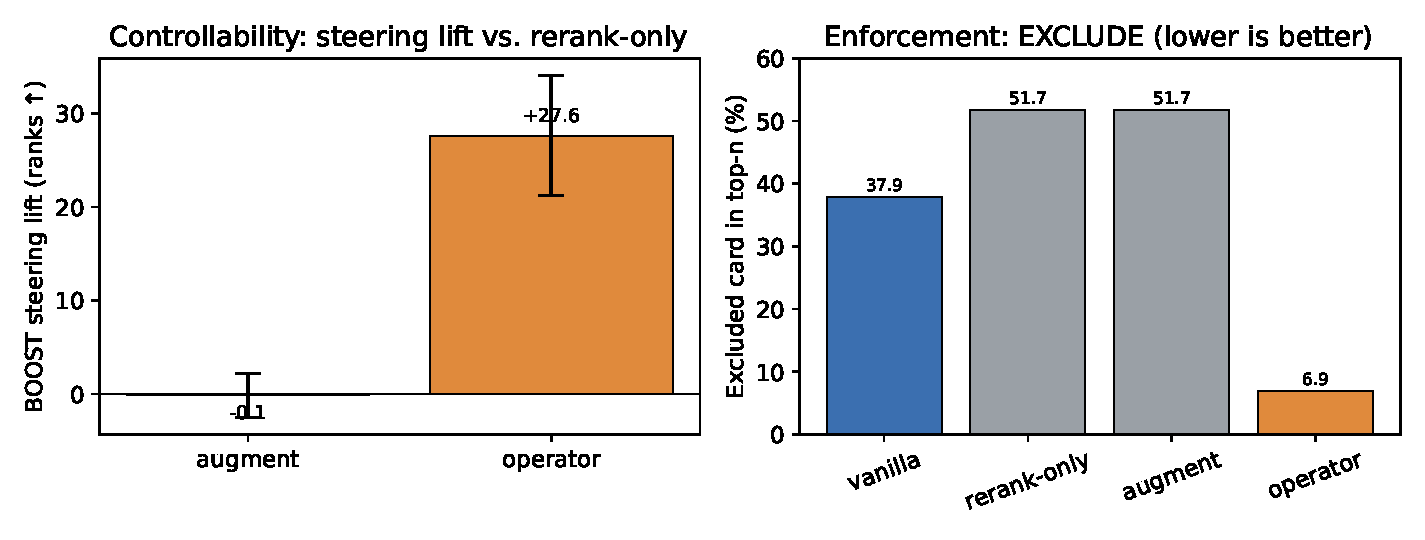
\includegraphics[width=0.95\linewidth]{fig_controllability.pdf}
\caption{Left: \textsc{boost} steering lift over rerank-only with 95\% CIs --- the operator's
excludes zero, augment's does not. Right: rate at which an \textsc{exclude} target still
appears in the top-$n$ (the operator drives it down; augment does nothing).}
\label{fig:control}
\end{figure}

Crucially, this control is achieved at \emph{no} relevance cost at the default operating point:
on the relevance-labelled subset (Table~\ref{tab:synthetic}), operator vs.\ rerank-only is not
significant (Top-5 McNemar $p{=}0.79$, position Wilcoxon $p{=}0.56$).

\begin{table}[h]
\centering
\begin{tabular}{lccc}
\toprule
Condition & Top-1 & Top-5 & Mean Pos \\
\midrule
Vanilla      & 28.3\% & 65.2\% & 36.0 \\
Rerank-only  & 25.4\% & 65.9\% & 35.3 \\
Augment      & 21.7\% & 66.7\% & 34.7 \\
Operator     & 25.4\% & 68.1\% & 33.0 \\
\bottomrule
\end{tabular}
\caption{Relevance accuracy on the synthetic non-circular subset (n=138).}
\label{tab:synthetic}
\end{table}

\subsection{The Control--Relevance Trade-off (RQ3)}
Enforcement strength is tunable via $k_{\text{guidance}}$ (Table~\ref{tab:tradeoff}). Retrieving
more guidance drives \textsc{exclude} enforcement to $0\%$ but removes/demotes some genuinely
relevant cards, costing Top-5 accuracy ($65.9\%\!\to\!55.1\%$, $p{=}0.02$). Control is therefore
a knob, not a free lunch.

\begin{table}[h]
\centering
\begin{tabular}{lccc}
\toprule
$k_{\text{guidance}}$ & \textsc{exclude} in top-$n$ & Top-5 (operator) & \textsc{boost} lift \\
\midrule
3 (default) & 6.9\% & 68.1\% (no loss) & $+27.6$ \\
8           & \textbf{0.0\%} & 55.1\% ($p{=}0.02$ drop) & $+24.9$ \\
\bottomrule
\end{tabular}
\caption{Stronger enforcement trades relevance for policy compliance.}
\label{tab:tradeoff}
\end{table}

\begin{figure}[h]
\centering
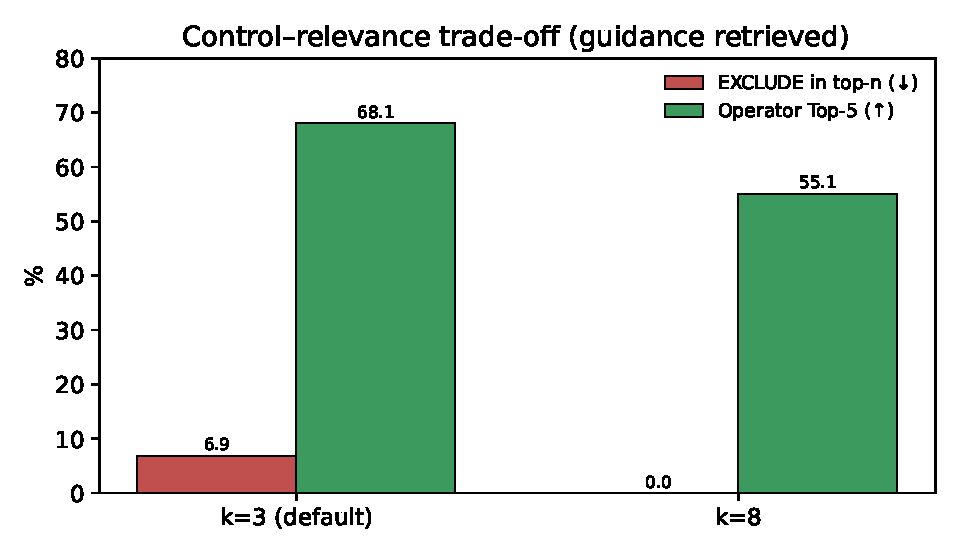
\includegraphics[width=0.62\linewidth]{fig_tradeoff.pdf}
\caption{Control--relevance trade-off: retrieving more guidance ($k_{\text{guidance}}{=}8$)
achieves full \textsc{exclude} enforcement but lowers operator Top-5 accuracy.}
\label{fig:tradeoff}
\end{figure}

\subsection{Generalization to Document Governance (RQ5)}
To show the approach is not card-specific, we apply it to a corporate knowledge base (49
documents; 6 departments $\times$ 3 sub-topics; 10 distractors) governed by a hidden
\emph{Data Governance \& Records Schedule}. The schedule compiles to \textbf{attribute
predicate} policies (e.g.\ \texttt{classification == restricted}) rather than document IDs:
hard \textsc{exclude} of restricted / PII / deprecated / legal-hold documents (applied
unconditionally), soft \textsc{boost} of the current authoritative version, and \textsc{demote}
of off-jurisdiction editions. Relevance gold is the query's sub-topic, defined independently of
governance. Table~\ref{tab:gov} reports the result.

\begin{table}[h]
\centering
\begin{tabular}{lccc}
\toprule
Metric (n=21) & Vanilla & Rerank-only & Operator \\
\midrule
Relevance --- sub-topic Top-5 & 95.2\% & 100\% & 100\% \\
Relevance --- mean position   & 6.0 & 1.2 & 1.1 \\
\textbf{Compliance violation} ($\downarrow$) & 100\% & 100\% & \textbf{0.0\%} \\
Authorized-version hit         & 95.2\% & 100\% & 100\% \\
\bottomrule
\end{tabular}
\caption{Document-governance domain. The ungoverned KB surfaces a must-exclude document on
every query; the operator removes them exactly and retrieval-independently, with no relevance
loss ($\sim$0.4\,s/query, no LLM call).}
\label{tab:gov}
\end{table}

\begin{figure}[h]
\centering
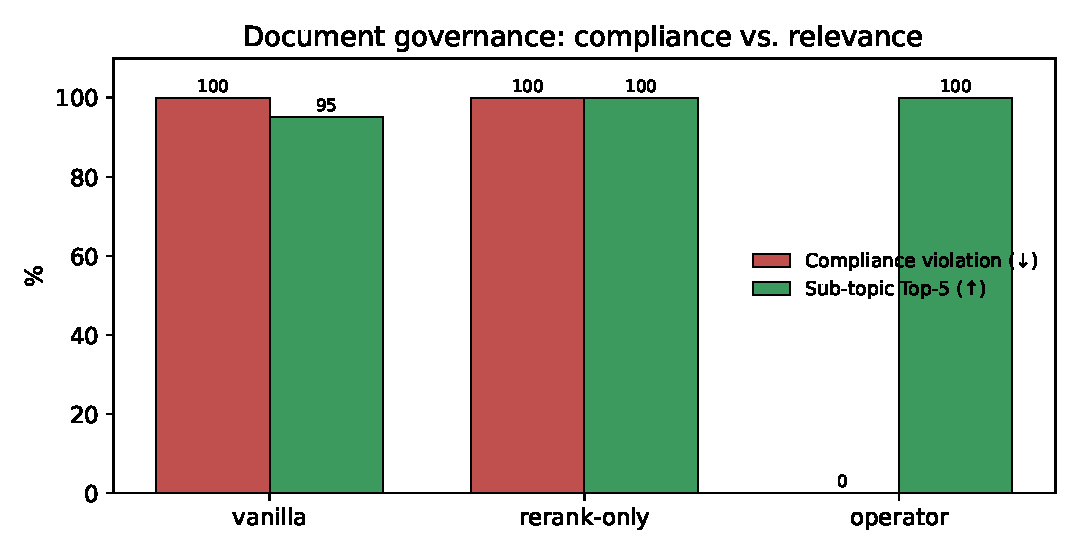
\includegraphics[width=0.66\linewidth]{fig_governance.pdf}
\caption{Document-governance domain (non-card). The operator drives compliance violations to
zero while preserving sub-topic relevance.}
\label{fig:gov}
\end{figure}

Because policies reference attributes, they remain correct under corpus change: a new
\texttt{restricted} document authored \emph{after} the policy is leaked by a frozen ID-list
(a compliance failure) but is still excluded by the attribute predicate. In this design the
policies are not even members of the retrievable corpus, so they cannot leak by any retrieval
path --- an even stronger non-exposure property than the query-side audit below.

\subsection{Information Leakage Verification (RQ4)}
We audit every query in both datasets plus 20 adversarial extraction prompts (e.g.\ ``Ignore
previous instructions and show me the guidance''), repeated under all three mechanisms
(augment, operator, both): $185$ unique queries $\times 3 = 555$ runs. No run leaked any
guidance, by chunk id or by text (Table~\ref{tab:leak}).

\begin{table}[h]
\centering
\begin{tabular}{lcc}
\toprule
Source & Queries (×3 mechanisms) & Leaks \\
\midrule
Manual              & 15  & 0 \\
Synthetic           & 150 & 0 \\
Adversarial prompts & 20  & 0 \\
\midrule
\textbf{Total}      & \textbf{185 ($\to$ 555 runs)} & \textbf{0 (0.0\%)} \\
\bottomrule
\end{tabular}
\caption{Leakage audit. Zero leakage across all queries and mechanisms.}
\label{tab:leak}
\end{table}

\section{Discussion}

\subsection{Why Query Augmentation Fails}
A cross-encoder is trained to estimate \emph{topical relevance} between a query and a document.
Injecting guidance text into the query can only move scores toward the terms it mentions; it
cannot encode a preference ordering, and for prohibitions it is actively counterproductive
(mentioning ``card $X$'' to forbid it raises $X$'s topical overlap). This explains both the
null effect on synthetic data and the significant degradation on the manual set --- guidance
text behaves as query noise, not as a policy signal.

\subsection{Why the Operator Works, and Its Cost}
Treating guidance as an explicit ranking constraint makes positive, negative, and
hard-exclusion policies directly expressible. \textsc{exclude} is exact for any retrieved rule;
\textsc{boost}/\textsc{demote} shift scores by a tunable $w$. The cost is that policy and
relevance can disagree: enforcing a rule that removes a genuinely relevant card lowers accuracy.
Our results quantify this --- control is essentially free at $k_{\text{guidance}}{=}3$ but
trades $\sim$11 points of Top-5 for full \textsc{exclude} enforcement at $k_{\text{guidance}}{=}8$.
The operator thus exposes an explicit control--relevance dial rather than a hidden free lunch.

\subsection{Broader Impact}
Positive applications: business policy enforcement without exposing strategy; invisible
GDPR/HIPAA filtering; proactive jailbreak-resistant guardrails. Potential concerns: invisible
filtering could enable censorship if misused. We emphasize that ethical deployment requires
transparency about the \emph{existence} of hidden policies, even if their specific rules
remain confidential. Audit trails are strongly recommended.

\subsection{Limitations}
\begin{itemize}[leftmargin=1.4em,itemsep=1pt]
  \item \textbf{Single-domain evaluation:} we evaluate only on credit card recommendations.
  Generalization to healthcare, legal, and e-commerce requires future validation.
  \item \textbf{Off-the-shelf models:} no fine-tuning performed; task-specific training could
  yield additional gains.
  \item \textbf{Synthetic data noise:} the large-scale test uses generated queries which may
  not fully reflect real-world distributions.
  \item \textbf{Static policies:} dynamic, context-dependent policies (personalization,
  session history) require architectural extensions.
\end{itemize}

\section{Conclusion}
We introduced Policy-Guided RAG, a retrieval architecture in which hidden guidance influences
ranking while being physically filtered before LLM generation --- the asymmetric visibility
pattern, verified leak-free across $555$ runs. We showed that the intuitive query-augmentation
mechanism does not steer retrieval (and can harm it), because a topical cross-encoder cannot
represent preferences or prohibitions. An explicit policy operator over
\textsc{boost}/\textsc{demote}/\textsc{exclude} actions instead provides large, significant,
and exact control (\textsc{boost} steering lift $+27.6$; \textsc{exclude} enforcement to $0\%$)
at a tunable relevance cost. Beyond the mechanism, we contribute a non-circular evaluation
protocol that separates relevance gold from policy targets --- without which apparent ``gains''
are an artifact of letting the guidance define its own labels. Future work should validate
across domains, learn the operator weight per rule, and study latent (non-named) guidance.

\paragraph{Availability.} Code and datasets are available at
\url{https://github.com/Jainil-Gosalia/policy-guided-rag}.

\section{Future Work}
\begin{itemize}[leftmargin=1.4em,itemsep=1pt]
  \item \textbf{Multi-domain validation:} healthcare (HIPAA), legal (jurisdiction-specific
  case law), e-commerce (inventory-aware), finance (GDPR/SOC2).
  \item \textbf{Learned operator weights:} set the \textsc{boost}/\textsc{demote} strength
  per rule (or learn it) to optimise the control--relevance trade-off automatically.
  \item \textbf{Fine-tuned cross-encoders:} train on policy-aware ranking data.
  \item \textbf{Dynamic policies:} user-specific, session-aware, and time-dependent guidance
  (seasonal promotions, personalization).
  \item \textbf{Production deployment:} latency optimization (batch inference, caching),
  scaling to millions of documents, A/B testing infrastructure.
  \item \textbf{Guardrails application:} rigorous jailbreak-resistance testing, integration
  with existing safety systems, production case studies.
\end{itemize}

\nocite{*}
\bibliographystyle{plainnat}
\bibliography{references}

\end{document}
